\documentclass[12pt,a4paper]{article}
\usepackage[utf8]{inputenc}
\usepackage[a4paper, margin=1in, bottom=1.5in]{geometry}
% San-seriff
% \usepackage{helvet}                       
% \renewcommand{\familydefault}{\sfdefault}
% San-seriff
\usepackage{mathptmx} %Time New Roman
\usepackage{fancyhdr}
% \usepackage{tabularx}
\usepackage{lastpage}
\usepackage{tabularray}
\UseTblrLibrary{booktabs}
\usepackage[dvipsnames]{xcolor}
\usepackage{titlesec}
\usepackage{titletoc}
\usepackage{fmtcount}
\usepackage{enumitem}
\usepackage{graphicx}
\usepackage[colorlinks=true, citecolor=black, linkcolor=black, urlcolor=blue]{hyperref}
% \usepackage[hidelinks]{hyperref}
\usepackage{csquotes}
\usepackage{parskip}
\usepackage{tabularx}
\usepackage{multirow}
\usepackage[table]{xcolor}
\usepackage{pifont} % checkmark

\definecolor{mygrey}{HTML}{d9d9d9}
\definecolor{headerblue}{HTML}{2F5597}
\definecolor{sectionbeige}{HTML}{F2E5C4}
\definecolor{rowgray}{HTML}{F7F7F7}

\titleformat{\section}[block]
  {\normalfont\Large\bfseries}
  {Chapter \Numberstring{section} \textbar}
  {0.5em}
  {}

\pagestyle{fancy}
\fancyhf{}
\renewcommand{\headrulewidth}{0pt}

\renewcommand{\contentsname}{TABLE OF CONTENTS}

\titleformat{name=\section,numberless}[block]
  {\normalfont\Large\bfseries\centering}
  {}
  {0pt}
  {}

\titlecontents{section}
  [0em]
  {\vspace{1ex}\bfseries}
  {Chapter \Numberstringnum{\thecontentslabel} \textbar\ }
  {}
  {\hfill\contentspage}

\titlecontents{subsection}
  [3em]
  {\normalfont}
  {\thecontentslabel\ }
  {}
  {\hfill\contentspage}

\titlecontents{subsubsection}
  [6em]
  {\normalfont}
  {\thecontentslabel\ }
  {}
  {\hfill\contentspage}

\setlength{\footskip}{31.45003pt}
\fancyfoot[C]{
    \footnotesize
    \begin{tblr}{
        width=\textwidth,
        colspec={|X[2.5,l]|X[3.5,l]|X[1.2,l]|X[1.5,l]|X[1.5,l]|X[2,l]|},
        hlines,
        vlines,
        column{1,3,5} = {bg=mygrey}
    }
    % Document Name & Converge\_Proposal\_v1.0.0 & Owner & PT, SP & Page & \thepage/\pageref{LastPage} \\
    Document Name & Converge\_proposal\_v1.0.5 & Owner & PT, SP & Page & \thepage/\pageref{LastPage} \\
    Document Type & Proposal & Release Date & 24-3-2026 & Print Date & - \\
    \end{tblr}
}

\usepackage{tabularray}
\UseTblrLibrary{booktabs}

\newcommand{\mytable}[2]{
\begingroup
\hbadness=10000
\noindent
\begin{tblr}{
    width=\textwidth,
    colspec={#1},
    hlines,
    vlines,
    row{1} = {bg=mygrey,font=\bfseries,halign=c},
    column{1} = {bg=mygrey,font=\bfseries,halign=c},
}
#2
\end{tblr}
\endgroup
}

\begin{document}

\begin{titlepage}
    \thispagestyle{empty}
    \centering
    \vspace*{3cm}
    {\Huge \textbf{Converge 4A}\par}
    {\Large Automated Appointment Arrangement Application\par}
    \vspace{1.5cm}
    {\Large \textbf{Project Proposal}\par}
    \vfill
    {\large Peeranat Thiwongsa 662115034\par}
    {\large Supawit Promma 662115049\par}
    \vspace{1.5cm}
    {\large Bachelor of Science\par}
    {\large Software Engineering Program\par}
    \vfill
    {\large College of Arts, Media, and Technology\par}
    {\large Chiang Mai University\par}
    {\large 3\textsuperscript{rd} Year\par}
    \vfill
    \rule{0.8\textwidth}{0.5pt}\par
    \vspace{0.8cm}
    {\large \textbf{Project Advisor}\par}
    \vspace{0.3cm}
    {\large Apitchaka Singjai, Dr.Techn.\par}
    \vspace*{1.5cm}
\end{titlepage}

\newpage
\setcounter{page}{2}

\section*{Document History}

\vspace{0.5cm}
\begingroup
\hbadness=10000
\noindent
\begin{tblr}{
    width=\textwidth,
    colspec={|X[0.7,c]|X[1.6,c]|X[0.6,c]|X[0.9,c]|X[0.8,c]|X[0.8,c]|},
    hlines,
    vlines,
    row{1} = {bg=mygrey,font=\bfseries},
}
Version & History & Status & Date & Editable & Reviewer \\
v0.1.0 & - Create Chapter 1,2 & C & 18-3-2026 & PT, SP & - \\
v0.1.0 & - Review Chapter 1,2 & R & 19-3-2026 & - & AS \\
v0.1.1 & - Update Chapter 1 & U & 22-3-2026 & PT, SP & - \\
v0.1.2 & - Update Chapter 2 & U & 23-3-2026 & PT, SP & - \\
v0.1.3 & - Create Chapter 3 & C & 23-3-2026 & PT, SP & - \\
v0.1.3 & - Review Chapter 1,2,3 & R & 23-3-2026 & - & AS \\
v0.1.4 & - Update Chapter 1,2,3 & U & 24-3-2026 & PT,SP & - \\
v0.1.4 & - Review Chapter 1,2,3 & R & 24-3-2026 & - & AS \\
v1.0.0 & - Update Chapter 1,2,3 & U & 24-3-2026 & PT,SP & - \\
v1.0.1 & - Update Chapter 1,2 & U & 16-4-2026 & PT,SP & - \\
v1.0.2 & - Update Chapter 1,2,3 & U & 17-4-2026 & PT,SP & - \\
v1.0.3 & - Update Chapter 1,2,3 & U & 18-4-2026 & PT,SP & - \\
v1.0.4 & - Update Chapter 1,2,3 and add risk management & U & 19-4-2026 & PT,SP & - \\
v1.0.5 & - Add SRS & U & 21-4-2026 & PT,SP & - \\
\end{tblr}
\endgroup

\vspace{0.5cm}
\noindent
*PT = Peeranat Thiwongsa \\
*SP = Supawit Promma \\
*AS = Apitchaka Singjai, Dr.Techn.

\vspace{0.5cm}
\noindent
\textbf{Version:} \\
document name vX.Y.Z \\
X: External published \\
Y: Test approval \\
Z: Internal review

\vspace{0.5cm}
\noindent
\textbf{Status:} \\
C = Create \\
R = Reviewed by advisor \\
U = Update \\
D = Delete

\newpage
\tableofcontents

\newpage
\section{Introduction and Rationale}
\subsection{Motivation}
Multi-branch tutoring centers operate in a highly dynamic environment where instructors frequently rotate between different branches to meet student demand. For these institutions, efficient scheduling is the operational backbone however, as the number of students, teachers, and physical branches grows, the complexity of coordinating weekly classes scales exponentially. Currently, administrators rely on manual systems to manage the schedule.

The booking process begins with a customer selecting a subject, followed by choosing a preferred instructor. The administrator must then manually filter through a static Excel spreadsheet to find and present that specific instructor's available time slots. If none of those times work for the customer, the administrator must repeat the entire filtering process for alternative instructors until a suitable time is found. Once a time is finally selected, the administrator acts as a middleman, sending a minimum of three separate LINE messages: first to the instructor to verify the requested slot, then back to the customer to finalize the booking, and finally to a staff group chat so the class can be manually logged.

When an instructor is booked for consecutive classes at different branches, administrators must manually calculate and block out their standard 30-minute commute buffer. Managing these transition times by hand across dozens of instructors significantly slows down the booking process. Furthermore, without a room tracking system, room availability is not guaranteed, leading to situations where teachers and students arrive at a branch only to discover that there is no physical room available.

Ultimately, this repetitive workflow consumes an estimated 1 to 2 hours of administrative time each day and introduces significant human error into the weekly recurring schedule, and forces administrators to manually cross reference multiple tables within a massive, cluttered spreadsheet just to find a single available teacher for a requested branch.

\subsection{Problem Statement}
% Administrators at multi-branch tutoring schools need an automated, commute-aware scheduling system because the current manual workflow wastes up to 2 hours of administrative time daily, it requires sending three messages per booking, relies on a cluttered spreadsheet that obscures operational insights, and results in room availability problem.
Administrators at multi-branch tutoring schools need an automated, commute-aware scheduling system because the current manual workflow wastes up to 2 hours of administrative time daily. The process requires sending at least three messages per booking, relies on a cluttered spreadsheet that obscures operational insights, and frequently results in room availability problems. To resolve this, the administration requires an algorithmic system capable of automatically evaluating inter-branch travel times and guaranteeing conflict-free resource allocation.

\newpage
\subsection{Purpose}
The primary purpose of the Converge application is to develop an automated scheduling and resource management system that eliminates the operational bottlenecks and inefficiency associated with manual booking in multi-branch tutoring centers. By replacing fragmented spreadsheet workflows and repetitive messaging with an intelligent, commute-aware engine, this project aims to provide administrators with a centralized platform to seamlessly align student requests, instructor availability, and physical room allocation in real-time.

\subsection{Target Users}
The target users of Converge are categorized into primary users, who interact directly with the scheduling interface, and secondary users, representing the organizations that benefit from the system's efficiency.

\subsubsection*{Primary Target Users}
\begin{enumerate}
    \item Administrator(Admin) are the primary operators who interact with the system daily to manage incoming requests from parents and input bookings into the interface. Their main objective is to finalize complex, multi-branch schedules in a matter of seconds while the customer is still present, ensuring a seamless and error-free experience. By using an automated system, they aim to eliminate the professional anxiety associated with manual errors, such as double-booking a room or taking an excessively long time to find an available slot, which can damage the school’s reputation
\end{enumerate}

\subsubsection*{Secondary Target Users}
\begin{enumerate}
    \item Parents and students act as secondary users who provide their subject preferences and availability to the administration in exchange for a reliable learning schedule. Their primary goal is to receive an immediate, 100\% accurate class confirmation—either printed or digital—without having to wait for a follow-up call. They are primarily driven by the fear of logistical failures, such as arriving at a branch for a scheduled lesson only to discover that the class was canceled, the room is occupied, or the instructor has not yet arrived due to a scheduling conflict.
\end{enumerate}

\newpage
\subsection{Project Scope}
% This project focuses on the design and development of Converge, a web-based scheduling and resource management system for multi-branch tutoring centers. The system aims to automate the booking workflow, optimize instructor scheduling across branches, and improve operational visibility by replacing manual spreadsheet-based processes:
% \begin{enumerate}
%     \item \textbf{Smart Booking Engine:} A constraint-based matching engine that evaluates tutor schedules, room capacities, and commute needed to present a calendar of all valid time slots. When a customer requests general availability rather than a specific tutor, the system automatically filters out all conflicting personnel and instantly presents the administrator with only the instructors capable of fulfilling the specific time and location requirements.
%     \item \textbf{Commute-Aware Scheduling:} A location-based constraint algorithm that automatically enforces a commute buffer when an instructor is assigned to consecutive classes at different physical branches. 
%     \item \textbf{Automatic Room Management:} A resource allocation module that dynamically assigns physical classrooms based on capacity and subject requirements to ensure that there is available room for each booking.
%     \item \textbf{Centralized Schedule Dashboard:} A unified, interactive web interface that allows administrators to view, manage, and modify daily operations across all branches in real-time. It replaces spreadsheets with a single source of truth, offering clear visual indicators of schedule conflicts and resource utilization.
% \end{enumerate}
This project focuses on the design and development of Converge, an enterprise-grade scheduling and resource management system utilizing heuristic optimization for multi-branch tutoring centers. The architecture replaces manual, error-prone workflows with an automated decision-support pipeline:
\begin{enumerate}
    \item \textbf{Automated Data Ingestion Pipeline:} Replaces unstructured manual schedule entry with a strict data validation layer, ensuring all instructor availability is normalized into discrete binary matrices before entering the database.
    \item \textbf{Symbolic AI Constraint Engine:} A backend algorithm that models tutoring logistics as a formal Constraint Satisfaction Problem (CSP). It mathematically guarantees conflict-free resource allocation by evaluating hard limits (tutor availability, room capacity) and soft constraints (schedule density).
    \item \textbf{Spatial-Temporal Routing (Commute Constraints):} A configuration-driven module that utilizes a customizable, admin-defined travel time matrix between branches. This instantly prunes the combinatorial search space to prevent impossible physical transit requirements without relying on external third-party geographic APIs.
    \item \textbf{Explainable AI (XAI) Decision Trace Dashboard:} An interactive administrative interface that exposes the heuristic scoring of the backend engine, allowing staff to rapidly understand algorithmic decisions and manually negotiate alternative times with clients based on clear logistical data.
    \item \textbf{Automated Disaster Recovery:} Scheduled, asynchronous database snapshot generation to ensure business continuity and data sovereignty for the B2B client.
\end{enumerate}
\textbf{Out of Scope}
\begin{enumerate}
    \item \textbf{Self-Service Client Booking Portal:} The client explicitly requires a manual, administrative-driven sales funnel to negotiate soft constraints and upsell packages to parents. Furthermore, following established research on Interactive AI in timetabling\cite{schaerf1999}, the system acts as an administrative decision-support tool rather than a fully automated "black-box" consumer app.
    \item \textbf{Payment Gateway and Financial Processing:} The client currently utilizes a proprietary, closed-source application for financial processing, which operates on a time-token ledger (where clients pre-purchase hours). Because this system lacks APIs for real-time balance inquiries and token deduction, Converge is architected strictly as a decoupled routing engine. Attempting to build fragile data-scraping workarounds to force state synchronization with a closed-source ledger introduces severe security risks—such as double-spending tokens or ledger corruption and is therefore strictly out of scope.
    \item \textbf{Probabilistic Machine Learning / Predictive AI:} The system utilizes deterministic Symbolic AI (Constraint Logic Programming) to guarantee mathematically exact schedules. It will not utilize statistical or generative AI (e.g., Large Language Models or predictive trend analysis), as guessing schedules introduces unacceptable logistical risks for physical resource allocation.
\end{enumerate}

\subsection{Feature Map (TODO)}
\vspace{0.5cm}
\begingroup
\hbadness=10000
\noindent
\begin{tblr}{
    width=\textwidth,
    colspec={X[l]|X[l]|X[0.6,l]|X[l]},
    hlines,
    vlines,
    row{1} = {bg=mygrey,font=\bfseries,halign=c},
}
Pain Point &
Feature Description &
Codename &
Success Metric \\
The manual booking workflow consumes an estimated 1 to 2 hours of administrative time daily. Furthermore, relying on a single, massive spreadsheet forces administrators to manually scan and cross reference complex tables to find an available instructor for a requested branch. &
A constraint-based engine that evaluates multiple variables to display valid slots. When specific instructors are not requested, the system acts as a smart filter to instantly present all qualified instructors who meet the strict time, room, and commute constraints. &
Auto-Pick &
Reduce average booking time to under 5 minutes per booking and eliminate the requirement for manual, middleman verification messaging.\\

Administrators struggle to manually calculate and block out cross-branch transit buffers (currently standardized at 30 minutes). &
A location-aware scheduling algorithm that automatically inserts mandatory travel buffers for consecutive cross-branch classes. &
Dynamic Buffer &
Fully automate the application of transit buffers.\\

The lack of room tracking leads to teachers and students arriving to find no physical classroom available. &
A room allocation system that treats physical classrooms as finite scheduling constraint. &
Auto-Allocate &
At most 4 instances of teacher/student arrive with no room available during the deployment phase.\\
The reliance on a Excel spreadsheet obscures operational insights and creates visual complexity. &
A unified web calendar interface that provides the Administrator with a clear, filtered view of every individual instructor's booked classes. &
Converge Hub &
Successfully migrate daily scheduling visibility from spreadsheets to a unified, real-time web dashboard.\\
\end{tblr}
\endgroup

\newpage
\section{Literature Review}
\subsection{Business Review / Software Review}
\subsubsection*{Calendly}
\begin{center}
    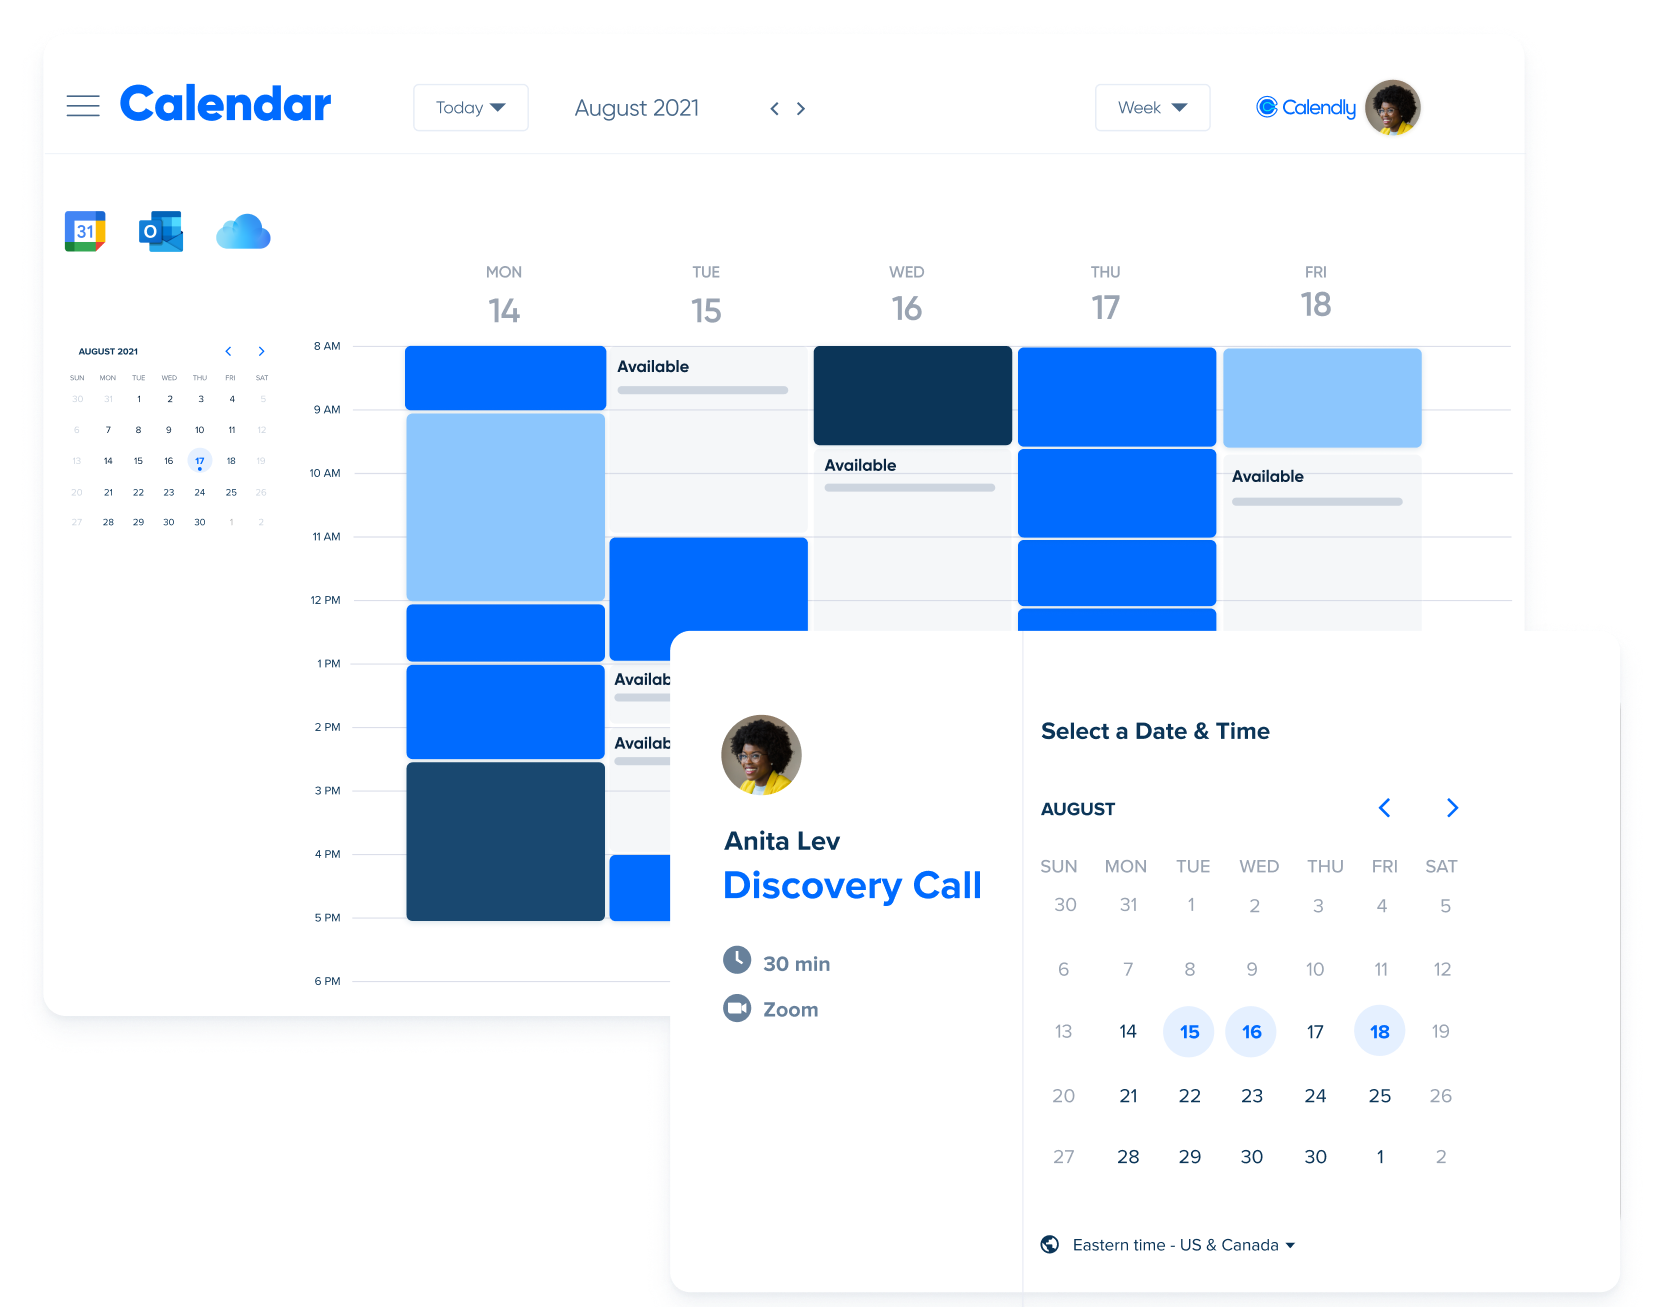
\includegraphics[width=0.7\textwidth]{images/CalendarConnections.png}
\end{center}
\textbf{Calendly}\cite{calendly_ref} is an automated scheduling platform that eliminates back-and-forth emails by allowing users to share their availability links, enabling invitees to instantly book open time slots.
\subsubsection*{Savvycal}
\begin{center}
    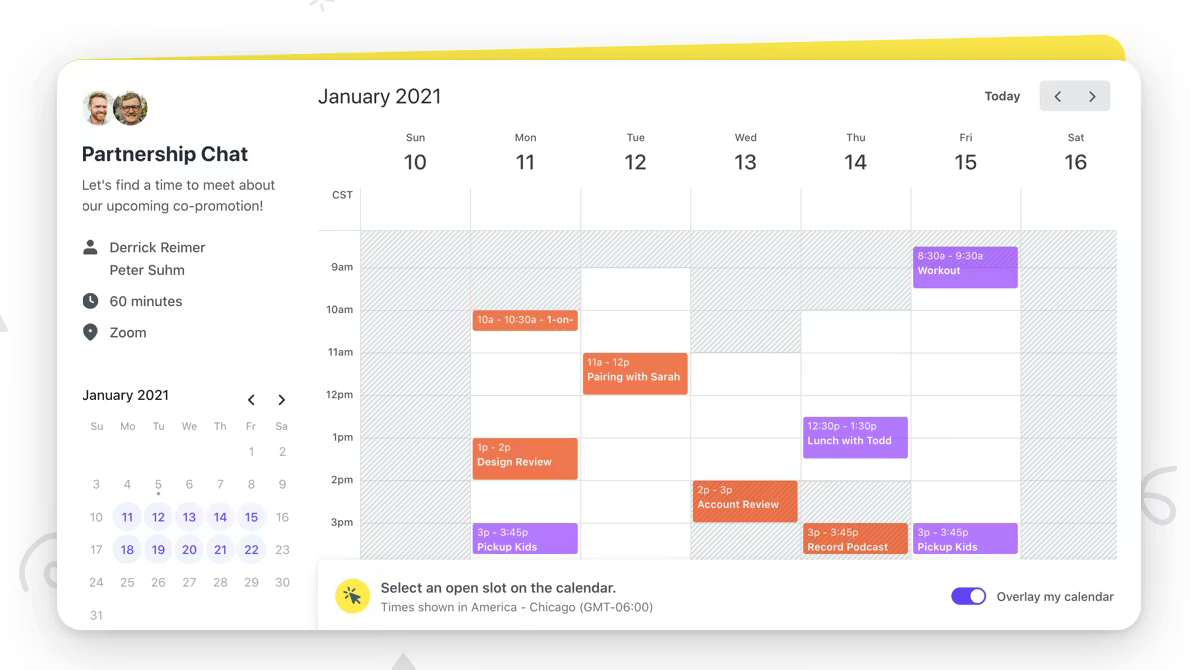
\includegraphics[width=0.7\textwidth]{images/Savvycall.png}
\end{center}
\textbf{Savvycal}\cite{savvycal_ref} is a collaborative scheduling tool featuring an interactive calendar overlay, which allows recipients to lay their own calendar over the sender's schedule to easily find mutual availability.
\subsubsection*{Doodle}
\begin{center}
    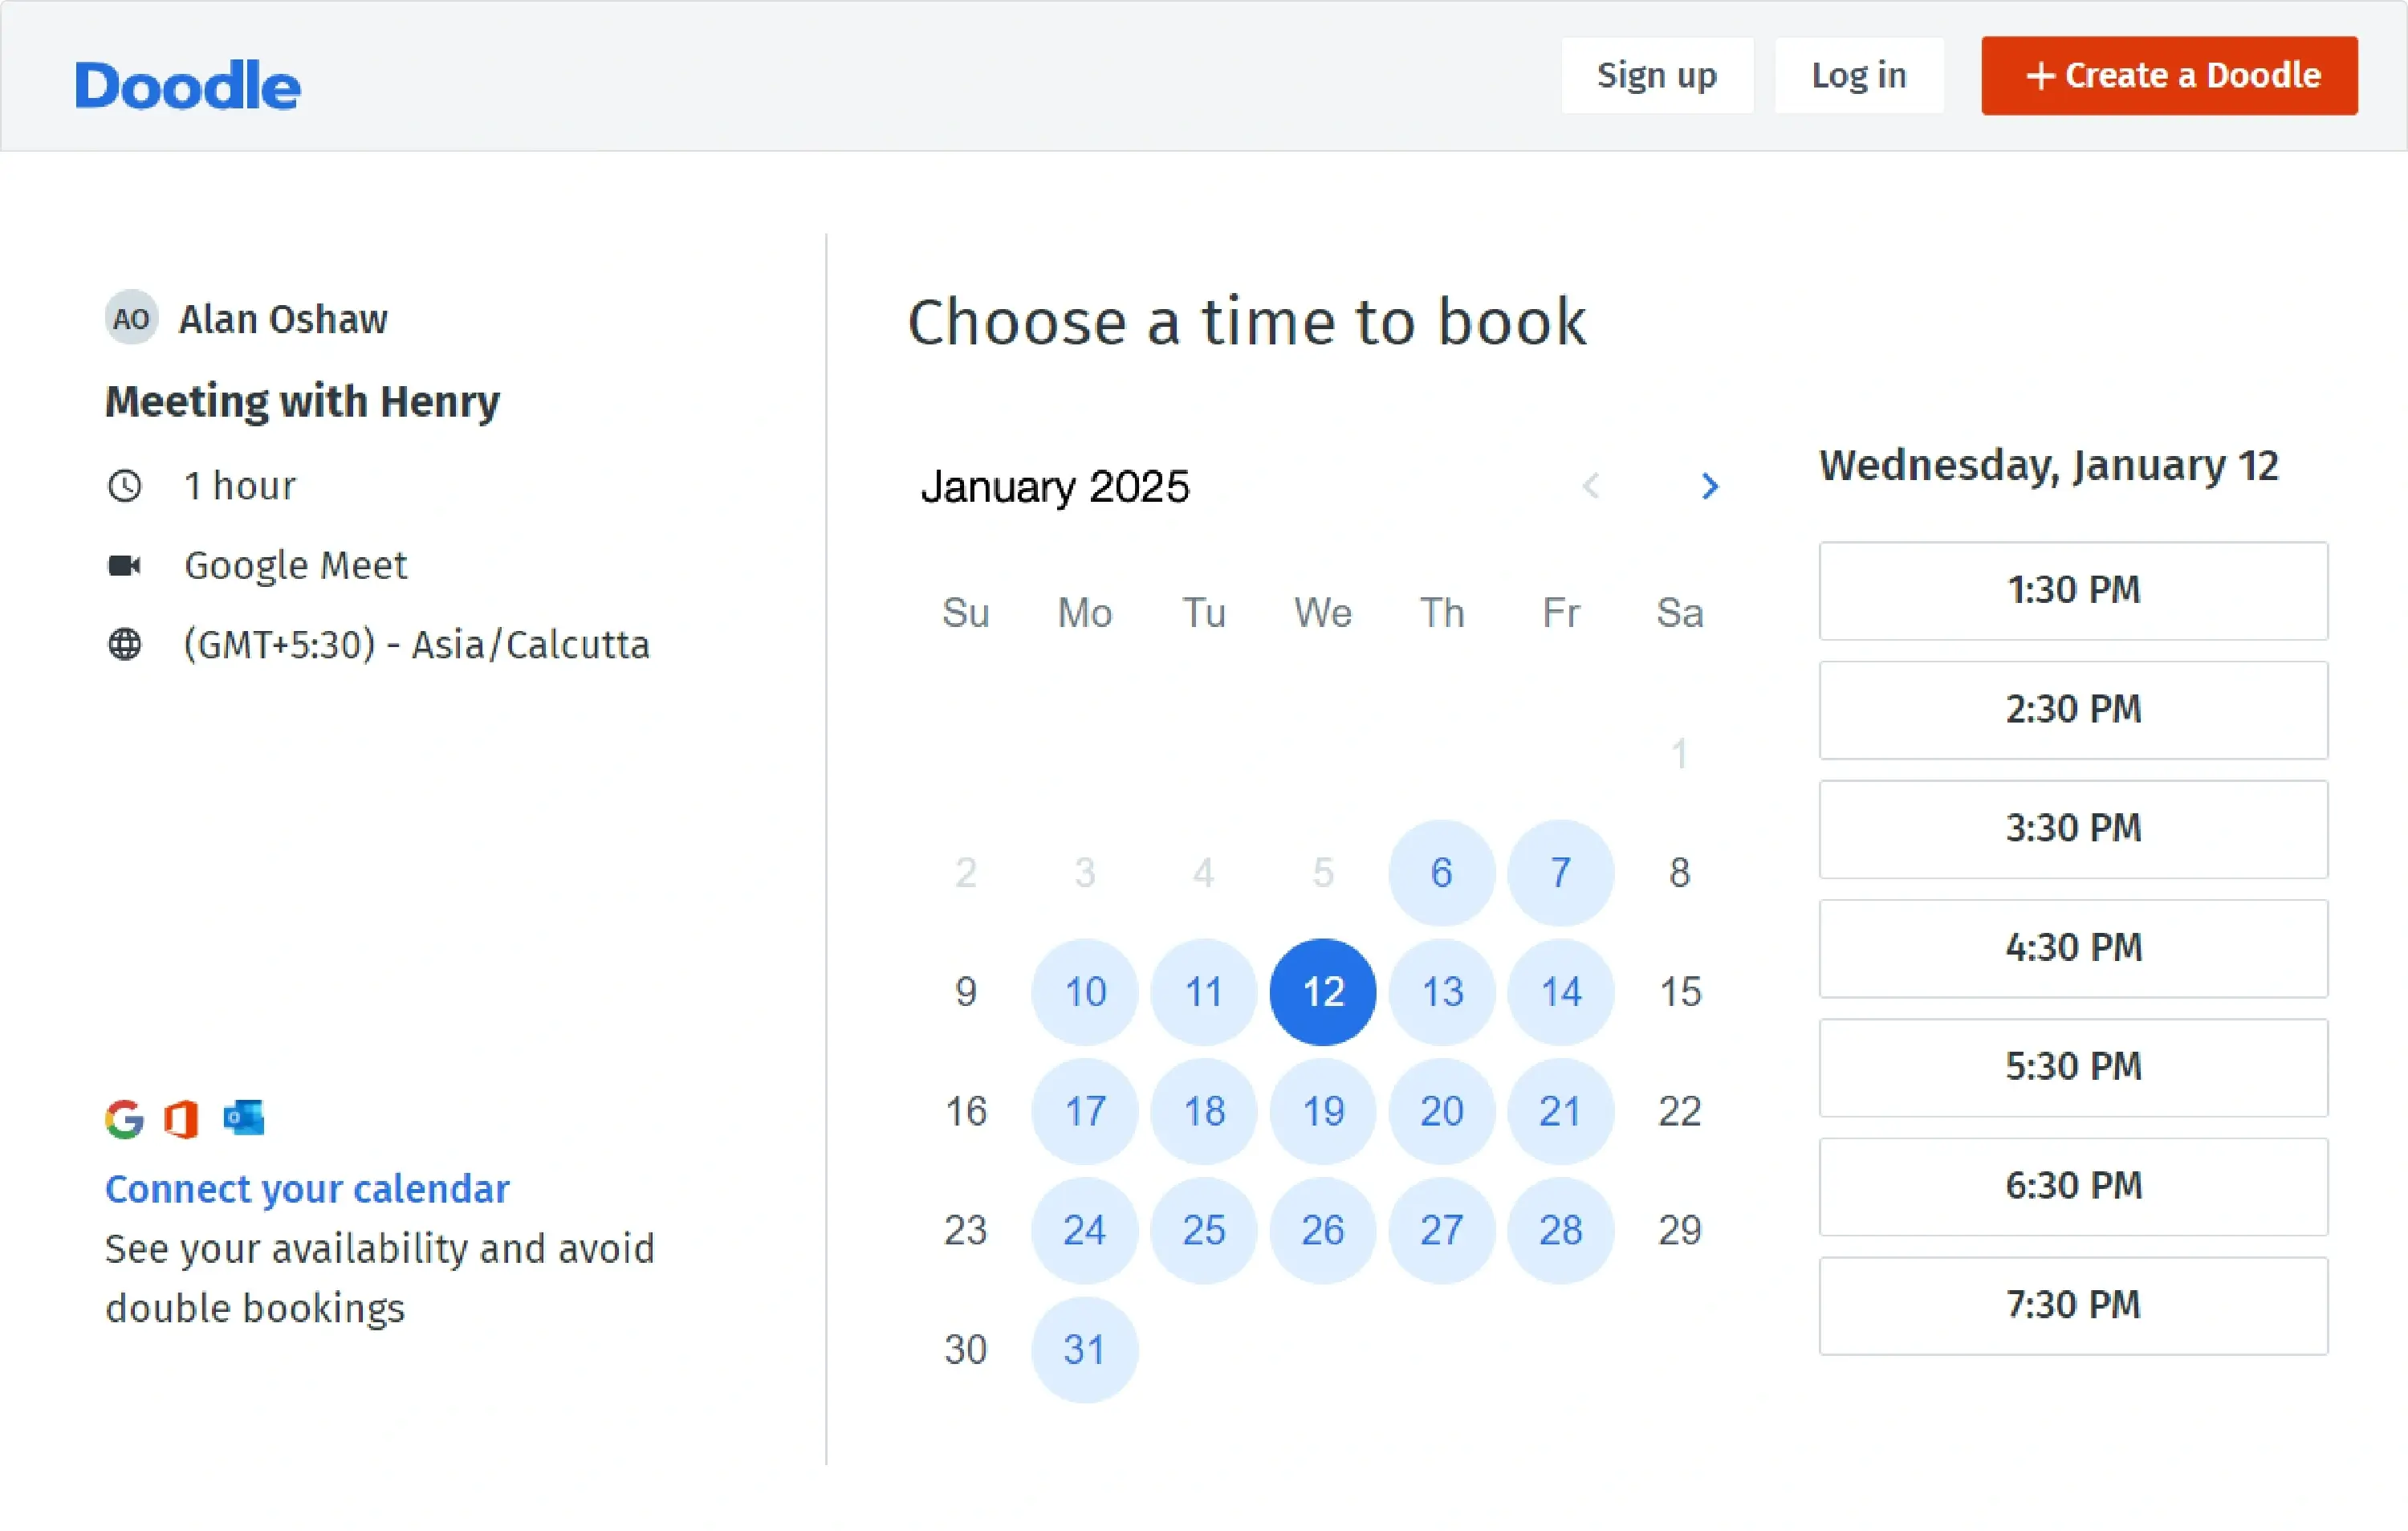
\includegraphics[width=0.7\textwidth]{images/doodle-img.png}
\end{center}
\textbf{Doodle}\cite{doodle_ref} is a group scheduling platform that utilizes a polling system, where an organizer proposes multiple time options and participants vote on their availability to determine the best consensus time for a meeting.

\subsubsection*{Comparative Table}
\vspace{0.5 cm}
\mytable{|X[1.5,l]|X[l]|X[l]|X[l]|X[1.5,l]|X[0.75,l]|}{
Feature & Calendly & Savvycal & Doodle & Converge \\

Smart Booking System & Partial — Link-Based  & Partial — Overlay-Based  & Partial — Consensus-Based  & Auto-Pick \\

Commute-Aware Scheduling & Partial — Fixed Buffers & Partial — Fixed Buffers & No — Not Supported & Dynamic Buffers \\

Automatic Room Management & Partial — Text-Only  & No — Not Supported  & No — Not Supported  & Auto-allocates  \\

Centralized Schedule Dashboard & NO — User-Centric & No — User-Centric & No — Event-Centric & Business - Centric \\
}

\newpage
\subsection{Architectural Foundations \& Prior Art}
Because generic SaaS tools fail to process spatial-temporal routing and multi-variable constraints, Converge abandons standard scheduling APIs. Instead, the system architecture is built upon established Operations Research and Artificial Intelligence methodologies to solve these specific logistical bottlenecks.
\subsubsection{Constraint Satisfaction Modeling for NP-Hard Problems}
Scheduling a distributed workforce across multiple physical locations is formally classified in computer science as an NP-hard optimization problem. If a standard brute-force algorithm attempts to examine every possible schedule combination, the time required to find a solution rises exponentially, leading to system failure at an enterprise scale.

To resolve this, the Converge core scheduling engine is modeled directly on Constraint Logic Programming (CLP) methodologies\cite{elsakka2015}. By formulating the tutoring schedule as a formal Constraint Satisfaction Problem (CSP), the architecture mathematically isolates hard constraints from soft constraints. The AI engine enforces strict physical realities such as ensuring an instructor is required only once at any given time point, and verifying that physical room occupancy does not exceed capacity before a schedule can be validated. This constraint-based approach guarantees mathematically conflict-free resource allocation without exhausting server memory.
\subsubsection{Spatial-Temporal Routing Constraints}
Generic SaaS scheduling applications are fundamentally ignorant of physical geography, relying entirely on simple temporal time-blocking. However, experience within the timetabling research community dictates that every single institution has its own unique rules, conventions, and operational fixations, rendering off-the-shelf software insufficient for specialized educational logistics\cite{ceschia2022}.

A critical requirement of the Converge architecture is the dynamic dispatching of personnel between physical branches. Addressing this requires a "rich formulation" that incorporates spatial-temporal routing constraints. As highlighted by recent state-of-the-art international timetabling benchmarks, such as the ITC-2019 dataset \cite{ceschia2022}, processing dynamic inter-branch travel times is a hallmark of complex real-world scheduling. Converge implements these findings by utilizing a customizable, pre-configured travel time matrix. By calculating commute buffers based on admin-defined durations between the instructor's previous and upcoming branches, the system instantly prunes invalid paths from the combinatorial search space to prevent impossible transit requirements.
\subsubsection{Heuristic Search and Interactive Explainable AI (XAI)}
When exact matches for student requests fail due to spatial-temporal or resource limitations, the system must calculate optimized alternatives. Because the search space is massive, the architecture implements Heuristic Search methodologies to rapidly score and return the next highest-scoring schedule vectors\cite{schaerf1999}.

Furthermore, fully automated "push-button" timetabling systems often fail in practice because human administrators require the flexibility to negotiate soft constraints directly with clients. Therefore, following Schaerf's findings on automated timetabling\cite{schaerf1999}, Converge is designed as an Interactive Decision Support System. The Symbolic AI engine processes the heavy spatial-temporal mathematics and exposes its logical trade-offs to the frontend via an Explainable AI (XAI) decision trace. This interactive architecture empowers administrative staff to manually finalize sales-driven booking decisions while relying on the backend engine to strictly enforce physical routing and capacity boundaries.

\subsection{Tool and Technology Review}
\subsubsection{Frontend Language}
\noindent
\begin{minipage}{0.15\textwidth}
    \centering
    
\includegraphics[width=1\linewidth]{images/TypeScript.png}
\end{minipage}
\hfill
\begin{minipage}{0.82\textwidth}
We chose \textbf{TypeScript}\cite{typescript_ref} over JavaScript as the frontend language because its compile-time error checking prevents structural logic failures in our multi-branch scheduling. In making this choice, we accept the tradeoff of a slower initial prototyping phase due to strict type definition requirements.
\end{minipage}
\vspace{0.5cm}\\
\mytable{|X[0.6,l]|X[l]|X[l]|X[l]}{
{Aspect / \\ Language} & TypeScript & JavaScript & Dart\\

Typing System & Static Typing & Dynamic Typing & Static Typing\\

Data Structure & Explicit Contracts & Flexible Objects & Classed Based Model\\

Development Tooling &
Strong IDE support &
Basic inference &
Strong Tooling\\

Trade Off &
High strictness overhead &
Risk of runtime errors &
Smaller Web Ecosystem \\
}

\subsubsection{Frontend Framework}
\noindent
\begin{minipage}{0.15\textwidth}
    \centering
    
\includegraphics[width=1\linewidth]{images/Vue.js.png}
\end{minipage}
\hfill
\begin{minipage}{0.82\textwidth}
We chose \textbf{VueJS}\cite{vuejs_ref} over React because its lower learning curve and built-in tooling allow us to focus on building features rather than configuring the project. In making this choice, we accept the tradeoff of a smaller ecosystem.
\end{minipage}
\vspace{0.5cm} \\
\mytable{|X[0.6,l]|X[l]|X[l]|X[l]|}{
{Aspect / \\ Framework} & VueJS & ReactJS & Angular \\

Component Structure &
Single File Component &
JSX &
Component + Template \\

State Management& 
Proxy-based &
Hooks &
Services + RxJS \\

Ecosystem & 
Small ecosystem (official tools) &
Massive ecosystem &
Large enterprise ecosystem \\

Trade Off &
Smaller community &
Steep learning curve &
Heavy framework, verbose \\
}

\newpage
\subsubsection{Backend Language}
\noindent
\begin{minipage}{0.15\textwidth}
    \centering
    \includegraphics[width=1\linewidth]{images/go.png}
\end{minipage}
\hfill
\begin{minipage}{0.82\textwidth}
We chose \textbf{Golang}\cite{golang_ref} over Java and NodeJS as the backend language because its compiled performance and native concurrency model perfectly balance raw execution speed with a low memory footprint. In making this choice, we accept the tradeoff of Go’s verbose syntax and manual error handling, which requires writing more boilerplate code than Node.js.
\end{minipage}
\vspace{0.5cm} \\
\mytable{|X[0.6,l]|X[l]|X[l]|X[l]|}{
{Aspect / \\ Language} & Golang & Java & NodeJS \\

Concurrency Model &
Native &
Thread-Based &
Single-Threaded \\

Execution Model &
Native Binary &
JVM Bytecode &
JIT Interpreted \\

Architecture &
Minimalist \& Explicit &
Strict OOP &
Highly Dynamic \\

Trade Off &
Verbose syntax &
High memory usage &
Potential bottlenecks \\
}

\subsubsection{Backend Framework}
\noindent
\begin{minipage}{0.15\textwidth}
    \centering
    
\includegraphics[width=1\linewidth]{images/gin.png}
\end{minipage}
\hfill
\begin{minipage}{0.82\textwidth}
We chose the \textbf{Gin}\cite{gin_ref} framework over Go’s native standard library (\texttt{net/http}) because its built-in routing and middleware capabilities significantly accelerate the development of our REST API. In making this choice, we accept the tradeoffs of framework lock-in and a slight memory overhead.
\end{minipage}
\vspace{0.5cm} \\
\mytable{|X[0.6,l]|X[l]|X[l]|X[l]|}{
{Aspect / \\ Framework} & Gin & net/http & Fiber \\

Routing &
Advanced &
Basic &
Express-style, fast \\

Middleware Management &
Built-in &
Manual &
Built-in \\

Data Binding \& Validation &
Automated &
Manual &
Limited \\

Ecosystem & 
Mature &
Minimal &
Growing \\

Trade Off &
Slight overhead \& lock-in &
More boilerplate &
Less standard, smaller ecosystem \\
}

\newpage
\subsubsection{Database}
\noindent
\begin{minipage}{0.15\textwidth}
    \centering
    
\includegraphics[width=1\linewidth]{images/PostgresSQL.png}
\end{minipage}
\hfill
\begin{minipage}{0.82\textwidth}
We chose \textbf{PostgreSQL}\cite{postgresql_ref} as the database because its native support for range data types is perfectly suited for a scheduling system. In making this choice, we accept the tradeoff of a steeper learning curve and slightly more configuration overhead.
\vspace{0.5cm} \\
\end{minipage}
\mytable{|X[0.6,l]|X[l]|X[l]|X[l]|}{
{Aspect / \\ Database} & PostgreSQL & MySQL & MongoDB \\

Data Model &
Relational &
Relational &
Document \\

Querying Complex Data &
Advanced &
Standard &
Aggregation-heavy \\

Data Type Support &
Range Types &
Basic Types &
Flexible Documents \\

Trade Off &
Steeper learning curve &
Limited advanced types &
Risk of inconsistency \\
}

\subsubsection{Architectural Pattern}
\noindent
\begin{minipage}{0.15\textwidth}
    \centering
    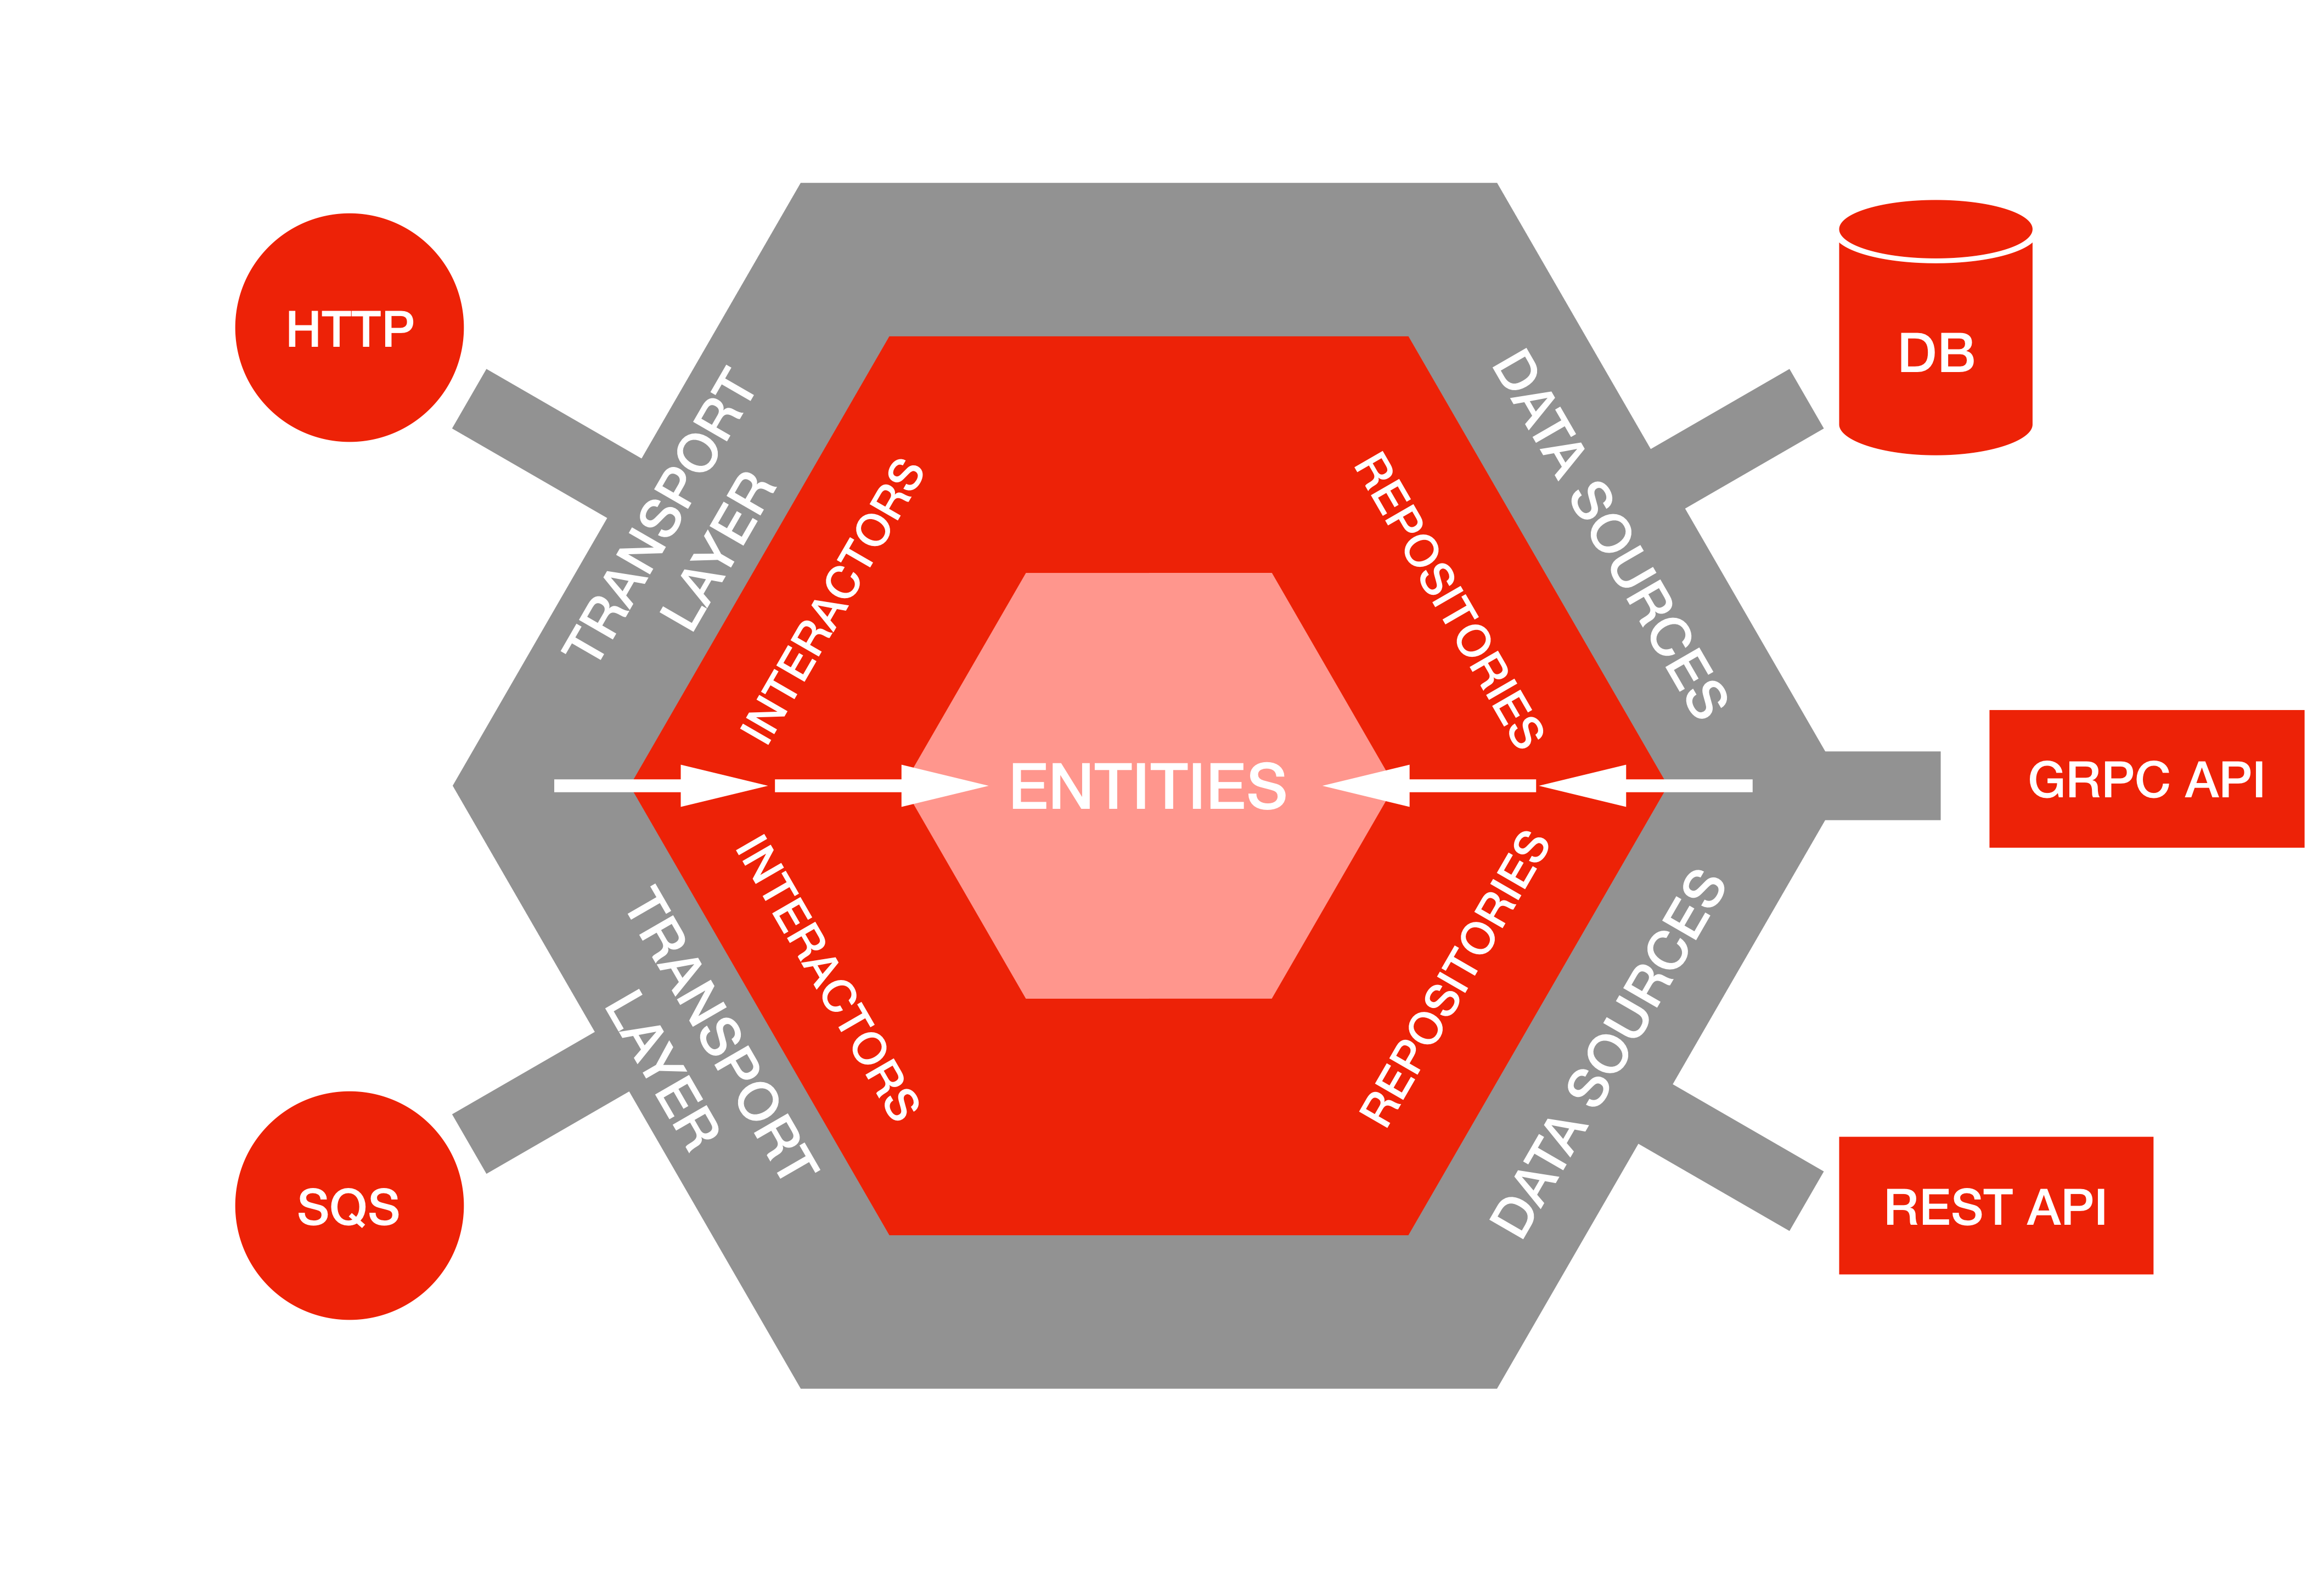
\includegraphics[width=1\linewidth]{images/hexagonal.png}
\end{minipage}
\hfill
\begin{minipage}{0.82\textwidth}
We chose \textbf{Hexagonal Architecture}\cite{hexagonal_ref} as the backend architectural pattern because it keeps the core scheduling domain portable and testable in isolation from the web framework. In making this choice, we accept the tradeoff of increased initial complexity, requiring more folders and interfaces upfront.
\end{minipage}
\vspace{0.5cm} \\
\mytable{|X[0.6,l]|X[l]|X[l]|X[l]|}{
{Aspect / \\ Architect} & Modular Monolith & Microservice & SOA \\

System Complexity &
Moderate &
High &
Moderate–High \\

Domain Modeling &
Well-structured &
Distributed &
Service-based \\

Operational Overhead &
Low &
High &
Moderate \\

Deployment &
Single deployable unit &
Independently deployable services &
Multiple services \\

Trade Off &
Requires discipline &
High infrastructure cost &
Less flexible than microservices, shared dependencies \\
}

\newpage
\subsubsection{Deployment Architecture}
\noindent
\begin{minipage}{0.15\textwidth}
    \centering
    
\includegraphics[width=1\linewidth]{images/modular_monolith.png}
\end{minipage}
\hfill
\begin{minipage}{0.82\textwidth}
We chose a \textbf{Modular Monolith}\cite{architecture_ref} over both Microservices and a standard Monolith to provide a safe evolution path for the system. This approach allows us to properly model the system using Domain-Driven Design (DDD) principles without the immediate operational complexity of a distributed network. In making this choice, we accept the tradeoff of relying on strict developer code discipline to enforce module boundaries, rather than relying on physical infrastructure separation.
\end{minipage}
\vspace{0.5cm} \\
\mytable{|X[0.6,l]|X[l]|X[l]|X[l]|}{
{Aspect / \\ Architect} & Modular Monolith & Microservice & Monolith \\

System Complexity &
Moderate &
High &
Low \\

Domain Modeling &
Well-structured &
Distributed &
Unstructured \\

Operational Overhead &
Low &
High &
Low \\

Trade Off &
Requires discipline &
High infrastructure cost &
Technical debt risk \\
}

\newpage
\subsubsection{Containerization}
\noindent
\begin{minipage}{0.15\textwidth}
    \centering
    
\includegraphics[width=1\linewidth]{images/Docker.png}
\end{minipage}
\hfill
\begin{minipage}{0.82\textwidth}
We chose \textbf{Docker}\cite{docker_ref} for containerization over traditional bare-metal because it guarantees environment consistency across development. By packaging the application and its dependencies into a single image, we eliminate environment-specific bugs. In making this choice, we accept the tradeoff of an increased learning curve, as the entire development team must understand Docker.
\end{minipage}
\vspace{0.5cm} \\
\mytable{|X[0.6,l]|X[l]|X[l]|X[l]|}{
{Aspect / \\ Strategy} & Docker & Podman & Bare Metal \\

Environment Consistency &
High  &
High  &
Variable \\

Resource Isolation &
High &
High &
Low \\

Deployment Speed &
Fast &
Fast &
Slow \\

Resource Overhead &
Low &
Low &
None \\

Security Model &
Daemon-based  &
Daemonless &
Host-dependent \\

Trade Off &
Requires daemon, slight overhead &
Less mature ecosystem &
Environment inconsistency \\
}

\newpage
\section{Project Plan}
% \subsection{Product Perspective}
\subsection{Objectives}
The primary objective of this project is to successfully design, develop, and deploy the Converge scheduling system. By the end of the development lifecycle, the project aims to achieve the following measurable goals:
\begin{enumerate}
    \item \textbf{Automate the Booking Workflow:} To drastically reduce the estimated 1 to 2 hours of daily administrative overhead  by replacing manual spreadsheet filtering and repetitive messaging with an automated matching engine.
    \item \textbf{Eliminate Scheduling Conflicts:} To implement a commute-aware algorithm and automated room allocation system that mathematically guarantees zero double-bookings and enforces realistic cross-branch travel buffers for instructors.
    \item \textbf{Enhance Operational Visibility:} To deliver a centralized, interactive web dashboard that provides business owners and administrators with a single, real-time source of truth for branch operations.
    \item \textbf{Implement a Scalable Architecture:} To engineer a robust backend utilizing a Modular Monolith and Hexagonal Architecture, ensuring the core scheduling domain is testable, highly maintainable, and prepared for future organizational scaling.
\end{enumerate}

\subsection{Type of System Users and the Users’ Characteristics}
\mytable{|X[0.2,c]|X[l]}{
{User Type} & Description \\

Admin &
the operators who manage course registrations and schedule bookings based on the incoming requests from parents.
\\

Parent &
the users who provide the subject that they want their child to learn to the admin.

} \\
\textbf{User Journey}
\begin{itemize}
    \item \textbf{As is:} A parent contacts the admin to book a class. The admin has to manually search through a cluttered Excel spreadsheet to find an open time slot. If the time works, the admin then has to manually calculate the teacher's travel time between branches and act as a middleman, sending multiple LINE messages back and forth to confirm with everyone. Even after all this manual work, they might arrive at the branch only to find no physical room is actually available.
    \item \textbf{To be:} A parent contacts the admin to book a class. The admin simply inputs the request into Converge. The system instantly auto-matches the available teacher and student , automatically adds the travel time for the teacher , and permanently locks in a physical room. The booking is confirmed accurately in seconds, completely cutting out the messy spreadsheets and group chats.
\end{itemize}

\subsection{Acronyms and Definitions}
\mytable{|X[0.2,c]|X[l]}{
Acronyms & Description \\

Admin &
The operators who manage course registrations and schedule bookings based on the incoming requests from parents.
\\

API &
\textbf{Application Programming Interface}\cite{api_ref}; used in the context of REST API for communication between the frontend and backend.
\\

Commute Buffer &
An automatically calculated travel time inserted between an instructor's consecutive classes at different physical branches.
\\

DDD &
\textbf{Domain-Driven Design}\cite{ddd_ref}; a software design approach focused on modeling the system based on the core business domain.
\\

Hexagonal Architecture &
A backend architectural pattern that keeps the core scheduling domain portable and testable in isolation from the web framework and database.
\\

Modular Monolith &
A deployment architecture where the system is deployed as a single unit but internally structured into well-defined modules.
\\

Parent &
The users who provide the subject that they want their child to learn to the admin.
\\

REST &
Representational State Transfer\cite{rest_ref}; the architectural style used for designing the system's web API.
\\

SaaS &
\textbf{Software as a Service}\cite{saas_ref}; a software distribution model mentioned as out-of-scope for this project.
\\

SDLC &
Software Development Life Cycle; the framework used for planning, creating, testing, and deploying the software.
\\

XP &
Extreme Programming; an Agile software development methodology focused on software quality, combined with Kanban for this project.
\\
}

\newpage
\subsection{System Architecture}
\textbf{1.Hexagonal Architecture}
\begin{center}
    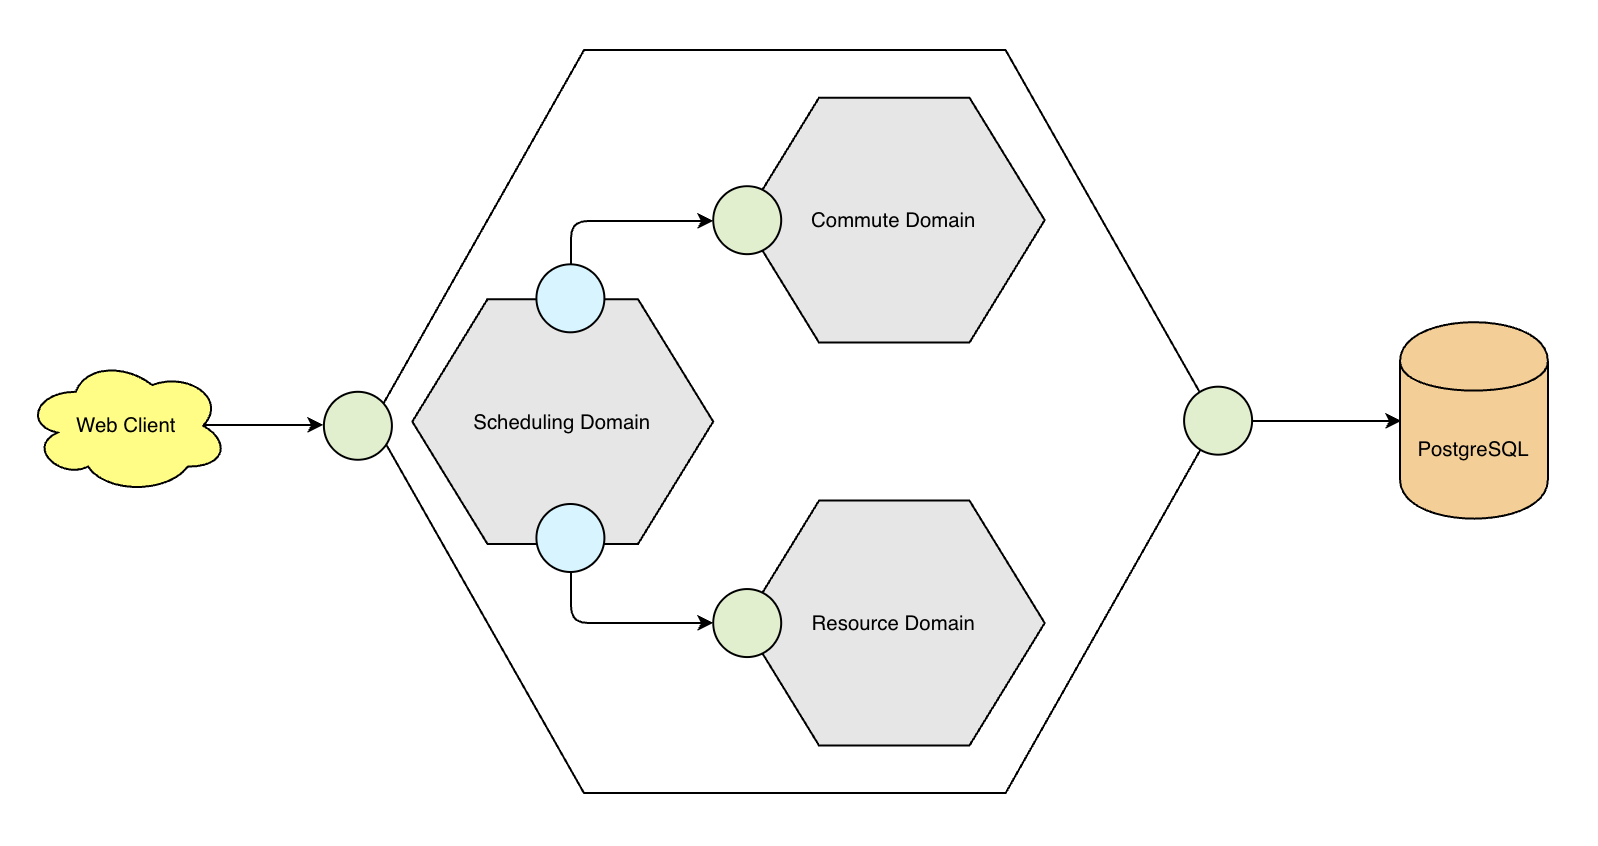
\includegraphics[width=1\textwidth]{images/converge_hexa.png}
\end{center}
\textbf{2.Modular Monolith Deployment Architecture}
\begin{center}
    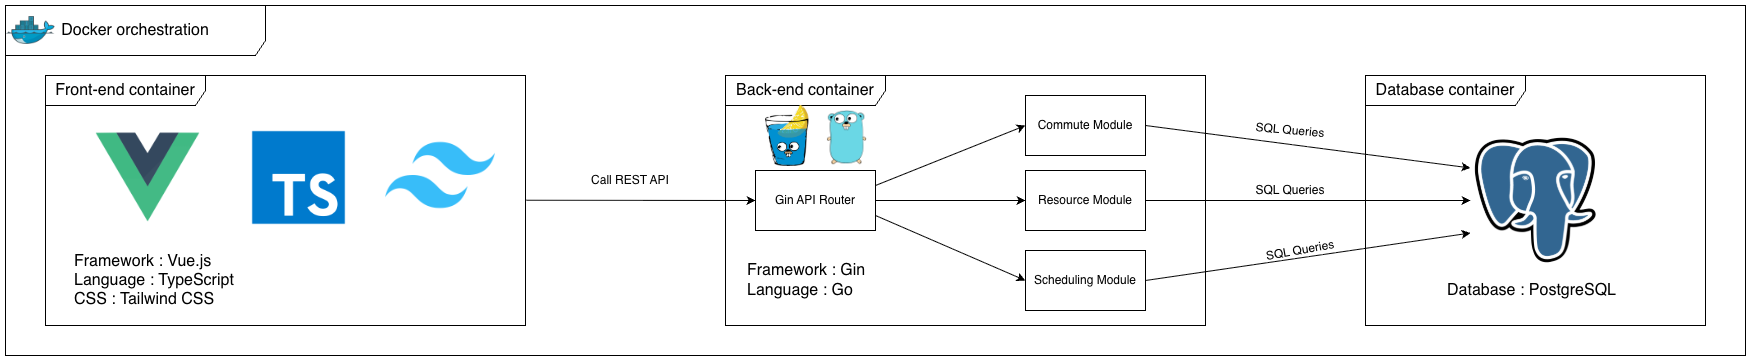
\includegraphics[width=1\textwidth]{images/converge_monolith.png}
\end{center}
\subsection{Use Case Diagram}
\begin{center}
    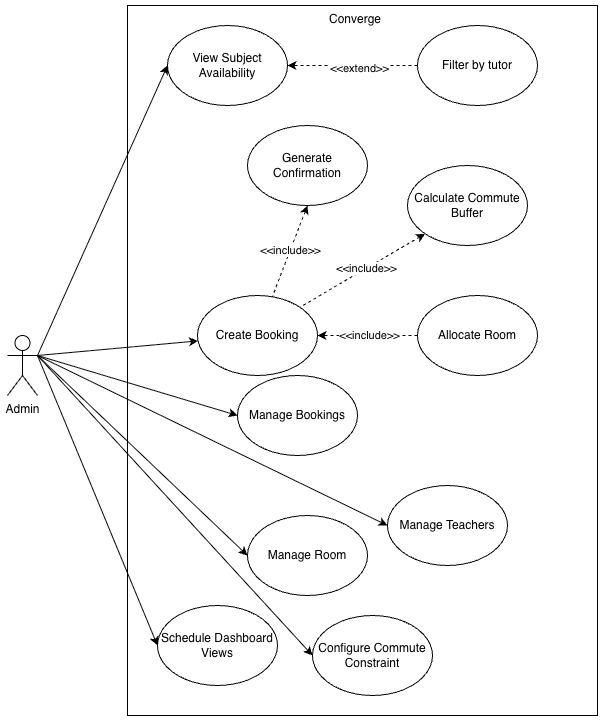
\includegraphics[width=1\textwidth]{images/converge_usecase.png}
\end{center}

\newpage
\subsection{Product Features}
\subsubsection{Smart Booking Engine}
\textbf{Description:} Automatically matches parent/student requests with valid instructors, time slots, and rooms. \\
\textbf{Actor:} Admin \\
\textbf{Details:}
\begin{itemize}
    \item \textbf{Request Input:}
    \begin{itemize}
        \item Admin must input subject and branch to initiate the search.
        \item Selection of a Preferred Time and Specific Instructor is optional, allowing the system to suggest all available possibilities.
    \end{itemize}
    
    \item \textbf{Constraint-Based Filtering:}
    \begin{itemize}
        \item Filters instructors based on availability, and subject expertise.
    \end{itemize}
    
    \item \textbf{Auto Suggestion:}
    \begin{itemize}
        \item Displays only valid booking options in real-time.
        \item Suggests alternative instructors or time if the specific request is unavailable.
    \end{itemize}
    
    \item \textbf{Booking Confirmation:}
    \begin{itemize}
        \item Automatically generates a digital summary of the finalized schedule once a booking is created.
    \end{itemize}
\end{itemize}

\subsubsection{Commute-Aware Scheduling}
\textbf{Description:} Enforces travel time whenever an instructor needs to change branch locations. \\
\textbf{Actor:} Admin \\
\textbf{Details:}
\begin{itemize}
    \item \textbf{Travel Buffer Enforcement:}
    \begin{itemize}
        \item Automatically shifts the next available start time forward by the fixed duration.
    \end{itemize}
    
    \item \textbf{Deterministic Logic:}
    \begin{itemize}
        \item Uses predefined travel times between branches or a default of 30 minutes.
    \end{itemize}
    
    \item \textbf{Visual Buffer Integrity:}
    \begin{itemize}
        \item The master schedule displays the commute as a specific \enquote{Travel Needed} making it clear to the administrator why a tutor's availability has been shifted.
    \end{itemize}
\end{itemize}

\newpage
\subsubsection{Automatic Room Management}
\textbf{Description:} Allocates and manages classroom resources automatically. \\
\textbf{Actor:} Admin \\
\textbf{Details:}
\begin{itemize}
    \item \textbf{Room Management:}
    \begin{itemize}
        \item Provides an interface to add new branch locations and modify rooms of existing branches.
    \end{itemize}

    \item \textbf{Branch Travel Configuration:}
    \begin{itemize}
        \item Provides an interface for administrators to define and modify custom travel times between specific branch pairs. Any pair without a custom value automatically falls back to the system-wide default of 30 minutes.
    \end{itemize}
    
    \item \textbf{Standardized Allocation:}
    \begin{itemize}
        \item Automatically pairs every booking with any available room at the target branch.
    \end{itemize}
    
    \item \textbf{Capacity Feedback:}
    \begin{itemize}
        \item Explicitly displays a \enquote{No Room Available} status for time slots where all physical spaces at a branch are already occupied.
    \end{itemize}
\end{itemize}

\subsubsection{Centralized Schedule Dashboard}
\textbf{Description:} Provides a unified interface to manage all schedules. \\
\textbf{Actor:} Admin \\
\textbf{Details:}
\begin{itemize}
    \item \textbf{Instructor Booking List:}
    \begin{itemize}
        \item Displays a structured list of all teachers and their complete set of booked classes across all dates.
    \end{itemize}
    
    \item \textbf{Alternative Visualizations:}
    \begin{itemize}
        \item Provides a toggleable calendar view as a visual alternative to the text-based assignment list.
        \item Displays commute buffers as explicit non-teaching blocks to ensure logging accuracy.
    \end{itemize}
    
    \item \textbf{Operational Filtering \& Management:}
    \begin{itemize}
        \item Enables filtering by specific instructor or branch.
        \item Includes the administrative interface for managing teachers and booking. 
    \end{itemize}
    
    \item \textbf{Commute Time Configuration:}
    \begin{itemize}
        \item Provides the interface for administrators to manage global system settings, such as modifying default commute constraints. 
    \end{itemize}
\end{itemize}

\newpage
\subsection{SDLC}
Based on our project scope and team size, we decided to use Agile methodologies. It is perfectly suited for a small, remote team like ours that is still in the learning phase and operating under short deadlines. Agile provides the exact flexibility we need to adapt and succeed.

After confirming Agile as our foundation, we chose to implement a Kanban + XP hybrid style. Kanban tells us what to work on next, while XP tells us how to write it well. Neither alone is enough, but together, they cover everything a 2-person remote team needs to deliver high-quality software.

Furthermore, we realized that a Continuous Flow (Kanban) fits our dynamics much better than fixed 2-week sprints. Since our team members have varying schedules and features naturally finish at different speeds, continuous flow allows us to pull work asynchronously without blocking each other's progress.

\subsection{Limits}
\begin{enumerate}
    \item \textbf{Administrative Access Only:} The system is designed as a back-office tool for center managers. It does not include a student-facing portal, tutor login accounts, or self-service booking interfaces for parents.
    \item \textbf{Non-Financial Scope:} The application does not handle any monetary transactions, including tuition fee collection, payroll processing for tutors, or tax invoicing.
    \item \textbf{No Automated External Notifications:} While the system calculates the optimal schedule, it does not send automated Email, or LINE messages. All communication with parents and tutors remains a manual process handled by the admin.
    \item \textbf{Fixed Time Commute Logic:} Commute buffers are calculated based on a configurable branch-pair matrix rather than real-time traffic data, eliminating dependency on external APIs. A default of 30 minutes applies to any pair without a custom value defined.
    \item \textbf{Single Organization Focus:} The architecture is designed for a single tutoring business with multiple physical branches. it is not a multi-tenant SaaS for multiple independent companies.
\end{enumerate}

\newpage
\subsection{Milestones}

\textbf{Phase 1: Proposal} — (30 March 2026 - 10 April 2026)\\
\mytable{|X[1.2,l]|X[l]|X[l]|X[l]|X[l]}{
Task & Start Date & End Date & Duration & Responsibility \\

Project Proposal & 
19 March 2026 &
10 April 2026 &
23 days &
PT, SP
\\

Topic defined &
19 March 2026 &
10 April 2026 &
23 days &
PT, SP
\\

Topic reviews &
21 March 2026 &
23 March 2026 &
3 days &
PT, SP
\\

Proposal submit &
24 March 2026 &
24 March 2026 &
1 days &
PT, SP
\\

Prepare for the presentation &
25 March 2026 &
29 March 2026 &
5 days &
PT, SP
\\

Proposal presentation &
30 March 2026 &
10 April 2026 &
12 days &
PT, SP
\\

Proposal submission &
24 April 2026 &
24 April 2026 &
1 days &
PT, SP
\\
}
\begin{center}
    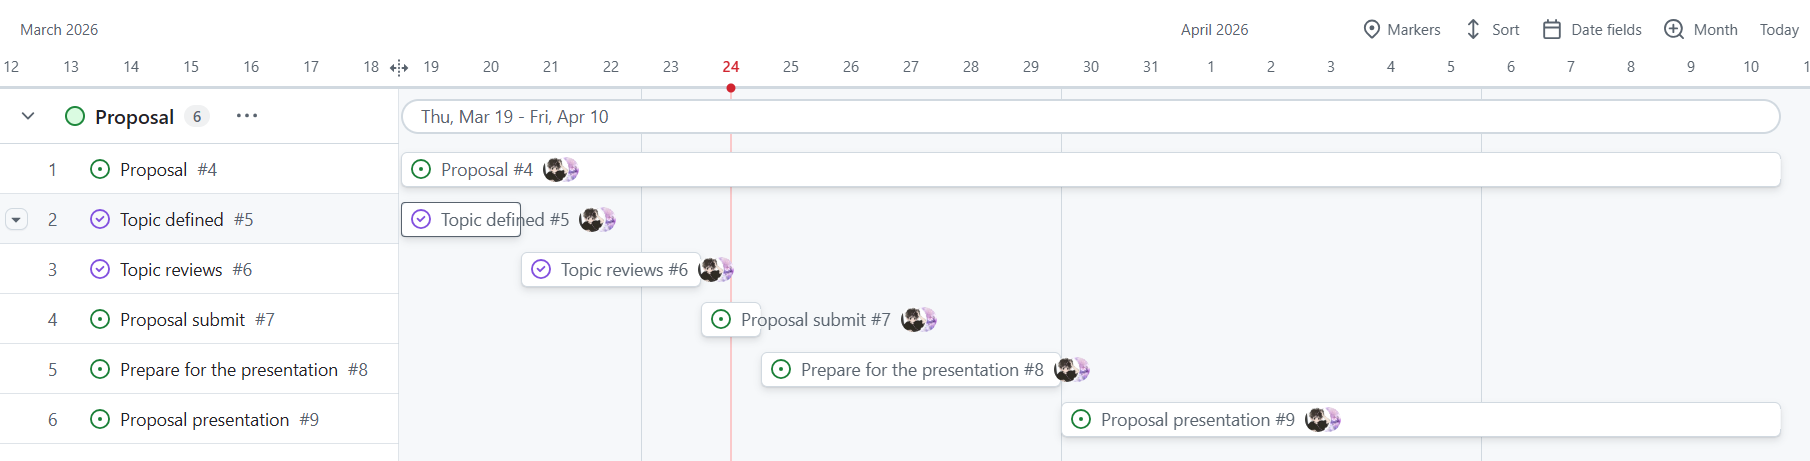
\includegraphics[width=1\textwidth]{images/timeline_proposal.png}
\end{center}

\newpage
\textbf{Phase 2: Progress I} — (15 April 2026 - 21 June 2026 2026)\\
\mytable{|X[1.2,l]|X[l]|X[l]|X[l]|X[l]}{
Task & Start Date & End Date & Duration & Responsibility \\

Setup Project Infrastructure &
15 April 2026 &
25 April 2026 &
11 days &
PT, SP
\\

Core Feature 1: Smart Booking Engine &
26 April 2026 &
25 May 2026 &
14 days &
PT, SP
\\

Core Feature 3: Automatic Room Management &
26 May 2026 &
12 June 2026 &
18 days &
PT, SP
\\

Prepare for Progress I &
13 June 2026 &
17 June 2026 &
5 days &
PT, SP
\\

Progress I Presentation &
18 June 2026 &
21 June 2026 &
4 days &
PT, SP
\\

}
\begin{center}
    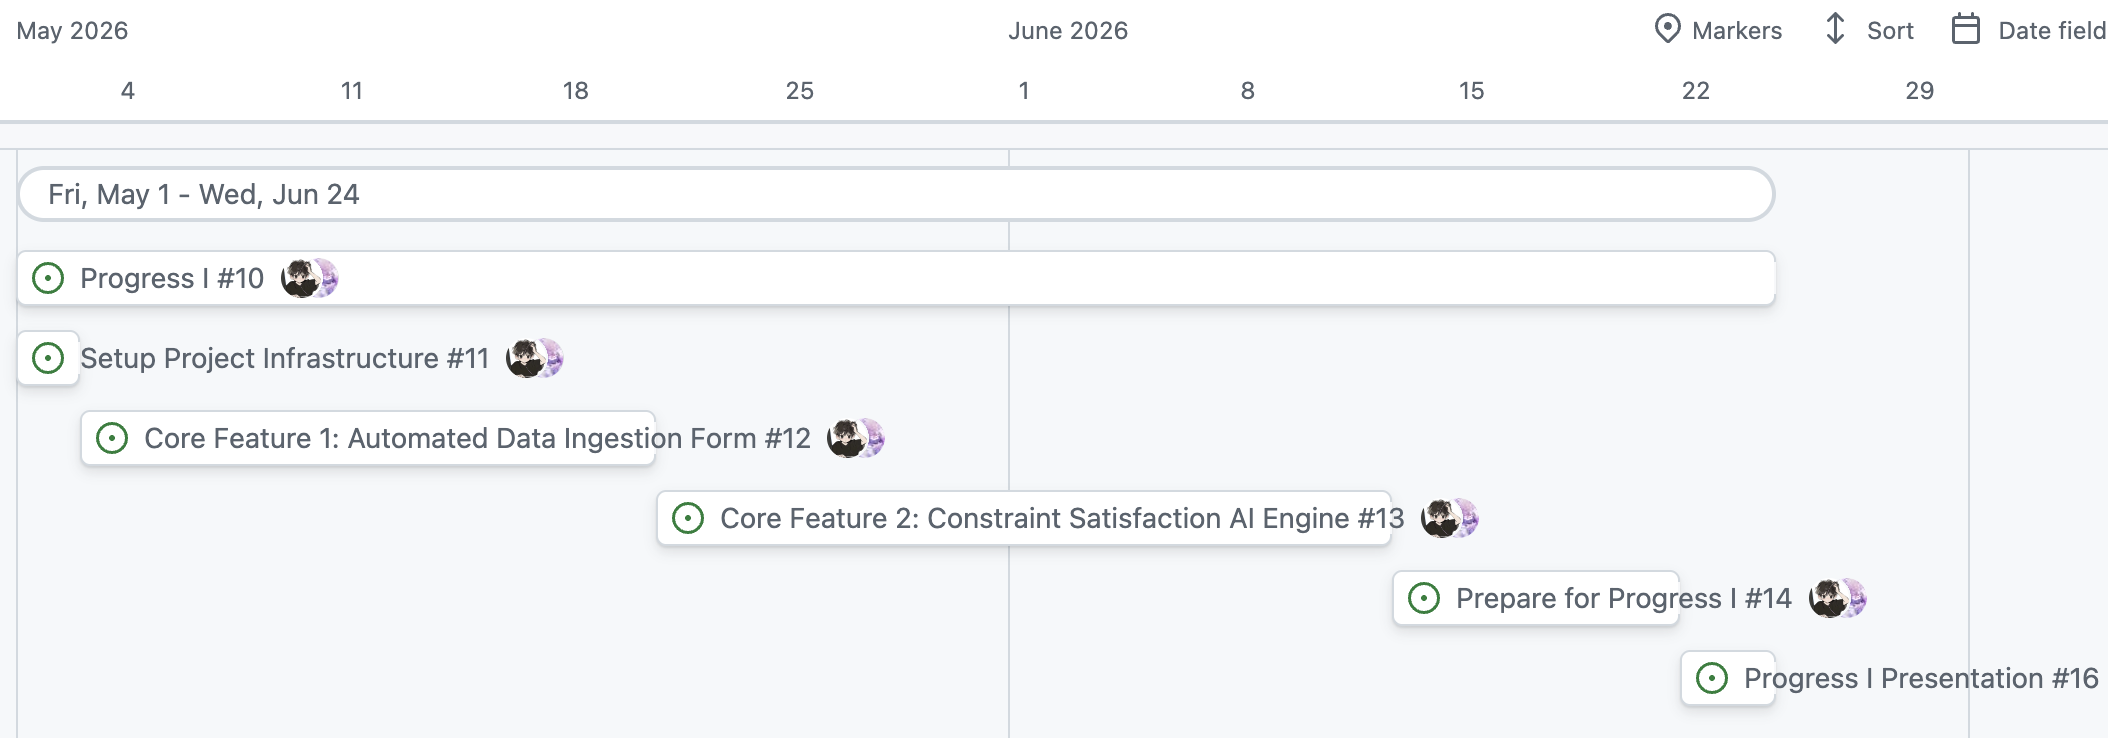
\includegraphics[width=1\textwidth]{images/progress1.png}
\end{center}

\newpage
\textbf{Phase 3: Progress II} — (22 June 2026 - 30 September 2026) \\
\mytable{|X[1.2,l]|X[l]|X[l]|X[l]|X[l]}{
Task & Start Date & End Date & Duration & Responsibility \\

Core Feature 3: Travel Buffer System &
1 July 2026 &
10 July 2026 &
10 days &
PT, SP
\\

Core Feature 4: Branch Capacity Monitoring &
11 July 2026 &
20 July 2026 &
10 days &
PT, SP
\\

Core Feature 5: Interactive XAI Decision Dashboard &
21 July 2026 &
30 July 2026 &
10 days &
PT, SP
\\

Core Feature 6: Automated Disaster Recovery &
31 July 2026 &
9 August 2026 &
10 days &
PT, SP
\\

Prepare for Progress II &
10 August 2026 &
16 August 2026 &
7 days &
PT, SP
\\

Progress II Presentation &
17 August 2026 &
21 August 2026 &
5 days &
PT, SP
\\
}
\begin{center}
    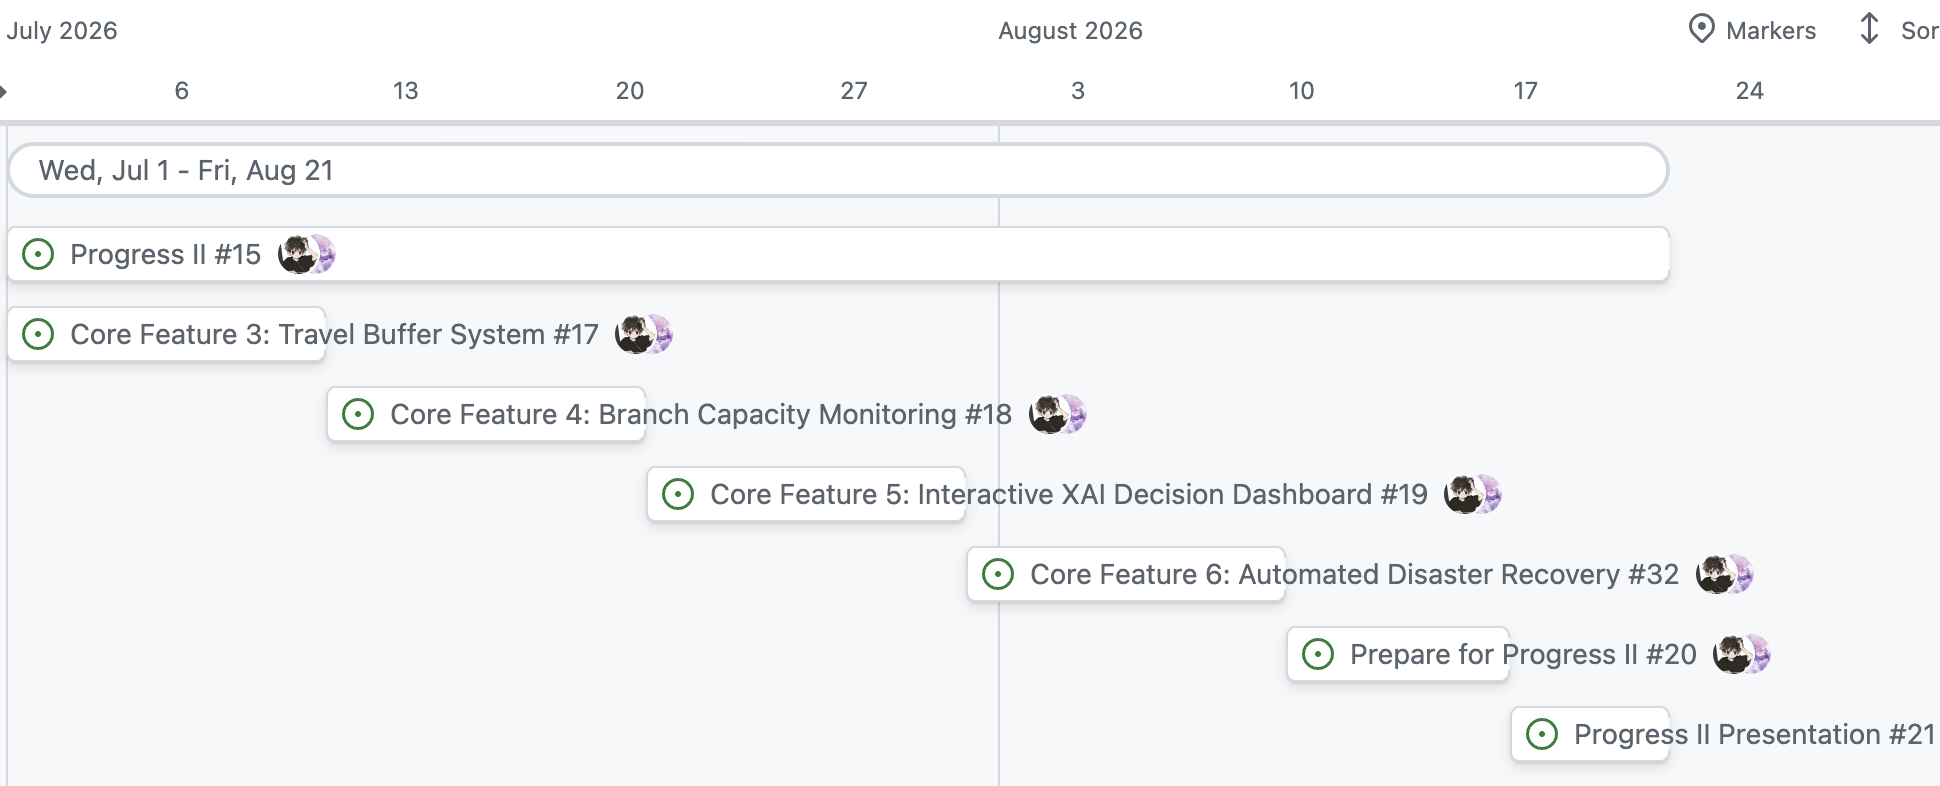
\includegraphics[width=1\textwidth]{images/progress2.png}
\end{center}

\newpage
\textbf{Phase 4: Final Progress} — (1 October 2026 - 2 November 2026)\\
\mytable{|X[1.2,l]|X[l]|X[l]|X[l]|X[l]}{
Task & Start Date & End Date & Duration & Responsibility \\

Quality Assurance &
1 October 2026 &
7 October 2026 &
7 days &
PT, SP
\\

System Documentation &
8 October 2026 &
14 October 2026 &
7 days &
PT, SP
\\

Prepare Final Presentation &
15 October 2026 &
18 October 2026 &
4 days &
PT, SP
\\

Final Progress Presentation &
19 October 2026 &
2 November 2026 &
15 days &
PT, SP
\\
}
\begin{center}
    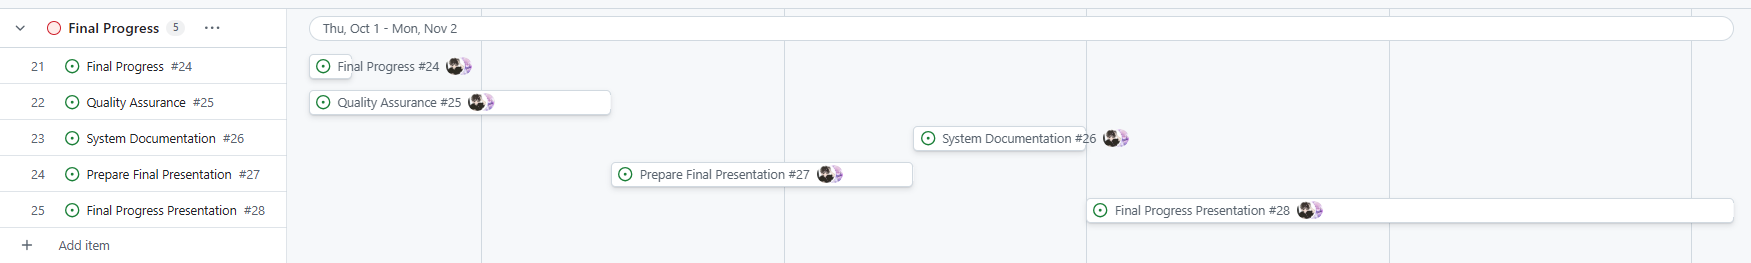
\includegraphics[width=1\textwidth]{images/final_progress.png}
\end{center}

\newcommand{\cmark}{\ding{51}}

\renewcommand{\arraystretch}{1.3}

\begin{tabularx}{\textwidth}{|X|c|c|}
\hline

\multirow{2}{*} 
& \multicolumn{2}{c|}{\textbf{Pct of task complete (\%)}} \\
\cline{2-3}
& \textbf{Progress I} & \textbf{Progress II} \\
\hline

\textbf{Feature 1: Automated Data Ingestion Form} & 0\% & 0\% \\
\hline

1.1 Structured Input &  & \\
1.2 Data Normalization&  & \\
\hline

\textbf{Feature 2: Constraint Satisfaction AI Engine} & 0\% & 0\% \\
\hline

2.1 Request Input &  & \\
2.2 Constraint-Based Filtering &  & \\
2.3 Heuristic Auto-Suggestion &  & \\
2.4 Explainable AI (XAI) Trace Logs &  & \\
\hline

\textbf{Feature 3: Travel Buffer System} & 0\% &  0\%\\
\hline

3.1 Buffer Configuration &  & \\
3.2 Deterministic Injection &  & \\
3.3 Visual Buffer Integrity &  & \\
\hline

\textbf{Feature 4: Branch Capacity Monitoring} & 0\% &  0\%\\
\hline

4.1 Capacity Definition &  & \\
4.2 Concurrent Tracking &  & \\
4.3 Capacity Feedback \& Prevention &  & \\
\hline

\textbf{Feature 5: Interactive XAI Decision Dashboard} & 0\% &  0\%\\
\hline

5.1 Master Schedule View &  & \\
5.2 Operational Filtering &  & \\
\hline

\textbf{Feature 6: Automated Disaster Recovery} & 0\% &  0\%\\
\hline

6.1 Asynchronous Snapshots &  & \\
6.2 Rapid Restoration &  & \\
\hline

\end{tabularx}

\newpage
\section{References}
\begingroup
\renewcommand{\section}[2]{}
\bibliographystyle{unsrt}
\bibliography{references}
\endgroup

\end{document}
